\documentclass[a4paper,12pt,twoside]{book}

\usepackage{polski}
\usepackage{fancyhdr} %naglowek i stopka
\usepackage[cp1250]{inputenc} %polskie znaki
\usepackage{graphicx} %wstawianie grafili
\usepackage{anysize} % do margines?w
\usepackage{indentfirst} %polskie "normy" akapitow
\usepackage{textcomp} %nazwisko czecha
\usepackage{afterpage}
\usepackage{amsthm}
\usepackage{float}

\pagestyle{fancy} 	
\fancyhead{} \fancyfoot{} 

\renewcommand{\chaptermark}[1]{\markboth{#1}{}}
\renewcommand{\sectionmark}[1]{\markright{\thesection\ #1}}

\fancyhead[RE,LO]{\normalfont \thepage}
\fancyhead[RO]{\normalfont \rightmark}
\fancyhead[LE]{\normalfont \leftmark}

\fancypagestyle{plain}{\fancyhead{}\renewcommand{\headrulewidth}{0pt}} 

\marginsize{3,5cm}{2,5cm}{2,5cm}{2,5cm}


\begin{document}
\tableofcontents
\chapter{Wst�p} \label{wstep} 
Celem poni�szej pracy jest zbudowanie autonomicznego pojazdu mobilnego, kt�ry konstrukcyjnie przypomina czo�g, w zwi�zku z czym wyr�nia si� nast�puj�cymi elementami:
\begin{itemize}
\item obrotow� wie�yczk� znajduj�c� si� na korpusie pojazdu,
\item dzia�em mog�cym zmienia� swoje po�o�enie.
\end{itemize}
Robot w spos�b autonomiczny stara si� zlokalizowa� przeciwnika. Po wykryciu zagro�enia czo�g stara si� okre�li� jego po�o�enie oraz odda� w jego stron� celny strza�. W ramach projektu nale�y : zbudowa� robota, wykona� projekt elektroniki, zaimplementowa� algorytm steruj�cy robotem, przeprowadzi� niezb�dne testy dzia�ana systemu oraz przygotowa� dokumentacj� techniczn�.

Koncepcja inteligentnych robot�w bojowych znajduje si� w kr�gu zainteresowa� s�u�b specjalnych takich jak wojsko czy policja. Pozwalaj� one przeprowadza� wiele niebezpiecznych operacji bez nara�ania �ycia za�ogi. Pokazdy bojowe - jako element wsparcia - nie mog� pope�nia� b��d�w zwi�zanych z b��dn� interpretacj� informacji, zatem podczas tworzenia projektu bardzo du�y nacisk b�dzie na�o�ony na algorytm przetwarzania pozyskanego obrazu otoczenia aby mo�liwie skutecznie oraz jednoznacznie zidentyfikowa� cel.  

\section{Za�o�enia kontrukcyjne}
Autonomiczne roboty mobilne musz� by� wyposa�one w system nawigacyjny. W naszym przypadku t� funkcj� b�dzie pe�ni� mikrokomputer wraz z kamer� video. Projekt oparty b�dzie o tzw. system wbudowany, czyli kompaktow�, multimedialn� jednostk� obliczeniow� wykorzystywan� do realizacji specjalnych funkcji takich jak sterowanie prac� silnika b�d� monitorowanie proces�w przemys�owych. Systemy wbudowane s� (najcz�ciej) na sta�e po��czone z elementami wykonawczymi oraz pomiarowymi. Najwa�niejsz� funkcj� czo�gu b�dzie przetwarzanie oraz analizowanie obraz�w w czasie rzeczywistym, co wymaga stosunkowo du�ej pami�ci oraz mocy obliczeniowej. Powy�sze wymagania pozwoli�y jednoznacznie wybra� platform�, na kt�re zrealizowany b�dzie projekt, mianowicie \textit{Raspberry Pi} wraz z dedykowan� kamer� \textit{Raspberry Pi Camera Board}.
Wyb�r modelu zawieszenia dla czo�gu jest jednoznaczny - g�siennice. Rozwi�zanie tego typu jest najcz�ciej spotykanym systemem jezdnym pojazd�w wojskowych. Roboty bojowe cz�sto zmuszone s� porusza� si� w bardzo zr�nicowanym i nieprzyjaznym �rodowisku. Stawia to przed uk�adem zawieszenia wiele wyzwa�.  G�siennice - dzi�ki r�wnoniernemu roz�o�eniu ci�aru (wiele pasywnych osi), du�ej powierzchni styku z pod�o�em, prostocie sterowania oraz trwa�o�ci s� niew�tpliwie najlepszym rozwi�zaniem w tej dziedzinie.
Ca�a konstrukcja nap�dzana b�dzie przy u�yciu silnik�w pr�du sta�ego. Sterowanie nap�dem b�dzie odbywa� si� przy u�yciu sygna�ow PWM generowanych przez \textit{Raspberry Pi} pozwalaj�cych na regulacj� pr�dko�ci obrotowej silnik�w.

\section{Budowa}
W strukturze robot�w mobilnych mo�emy wyr�ni� nast�puj�ce elementy :
\begin{enumerate}
\item 
Baza pojazdu~:
	\begin{itemize}
	\item
	konstrukcja mechaniczna pozwalaj�ca na pokonywanie nier�wno�ci terenu, 
	\item 
	uk�ad zasilania i sterowania silnikami robota,
	\item 
	modu�y pomiarowe pozwalaj�ce analizowa� otoczenie w jakim si� znajduje,
	\item
	komunikacja z systemem nadzoruj�cym prac� pojazdu.
	\end{itemize}
\item
Komputer PC, do kt�rego trafiaj� wszystkie informacje zebrane z czujnik�w. Jego zadaniem jest dok�adna analiza otoczenia robota, podj�cie decyzji co do dalszych ruch�w oraz realizacja zaplanowanego zadania. 
\end{enumerate}


\chapter{Stan obecnej wiedzy}
\section{Rozw�j robotyki}
M�wi si� �e, �e robotyka jest owocem wszystkich dotychczasowych osi�gni�� ludzko�ci w ka�dej dziedzinie. ��czy w sobie przede wszystkim elementy : mechaniki, automatyki, elektroniki, sensoryki oraz cybernetyki.
Jej poszczeg�lne elementy by�y rozwijane na przestrzeni setek a nawet tysi�cy lat. Pierwsze wzmianki historyczne dotycz�ce budowy robot�w si�gaj� oko�o 350 roku p.n.e. i dotycz� greckiego matematyka Archtasa z Tarentu, kt�ry rzekomo zbudowa� ptaka nap�dzanego spr�onym powietrzem oraz potrafi�cego lata�. Niestety ale zweryfikowanie tej wiadomo�ci jest bardzo skomplikowane i nie daje jednoznacznej odpowiedzi. Wskazuje ona jednak na zainteresowanie ludzko�ci budow� maszyn-robot�w, kt�re pierwotnie mia�y na�ladowa� natur�. Za pocz�tek rozwoju robotyki uwa�a si� prze�om XV oraz XVI wieku, w kt�rym za spraw� wielkiego wynalazcy - Leonadra da Vinci powsta�o wiele interesuj�cych projekt�w oraz konstrukcji. Jego wizje niejednokrotnie znacznie wykracza�y poza czasy, w kt�rych �y�. Na ilustracji \ref{czolg_leon} przedstawiony zosta� szkic przedstawiaj�cych jedn� z zaprojektowanych przez Leonarda maszyn wojennych - przodek wsp�czesnego czo�gu, kt�ry mia� miota� kamienie oraz by� nap�dzany si�� ludzkich mi�ni.

\begin{figure}[h] \label{czolg_leon}
\centering
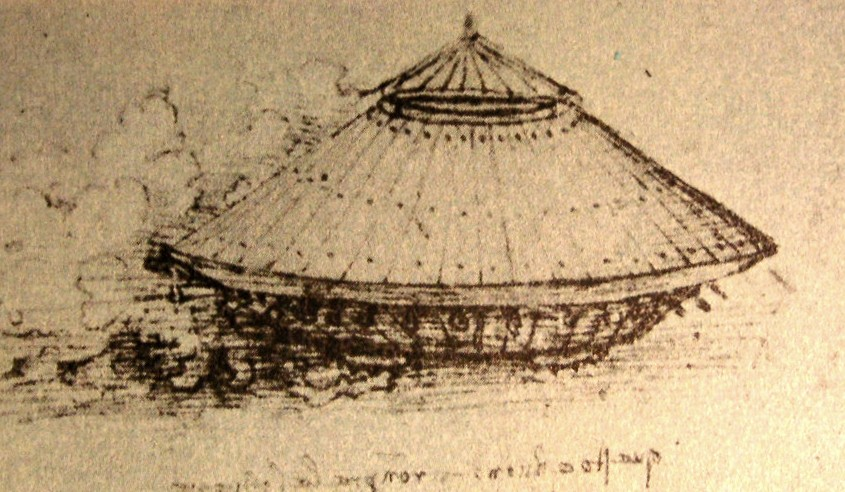
\includegraphics[scale=0.3]{imgs/Leonardo_tank.jpg}
\caption{Szkic Leonarda da Vinci przedstawiaj�cy jego koncepcj� czo�gu.}
\end{figure}

Kolejny prze�om w tej dziedzinie przypada na po�ow� XVIII wieku, w kt�rej to francuz Jacques de Vaucanson buduje swoje automaty. Z jego licznych konstrukcji pragn� wyr�ni� 3 najbardziej znane, tzn. : mechaniczny ch�opiec graj�cy na flecie, mechaniczny ch�opiec dodatkowo graj�cy na tamburynie, mechaniczn� kaczk�, potrafi�c� porusza� si�, wydawa� odg�osy, porusza� skrzyd�ami oraz symulowa� uk�ad trawienny.

Jednak�e prawdziwy prze�om w robotyce dokonuje si� w 1821 roku, w kt�rym Michael Faraday zbudowa� pierwszy silnik elektryczny, kt�rego dalszy rozw�j wywar� ogromny wp�yw na koncepcj� konstrukcji robot�w. Mechaniczne (np. spr�yny) oraz chemiczne (spalanie paliw) �r�d�a energii b�d� powoli wypierane z tej dziedziny nauki na rzecz rozwi�za� elektrycznych, pozwalaj�cych na prostsze, bezpieczniejsze oraz wydajniejsze magazynowanie oraz bardziej elastyczne wykorzystanie.

Upowszechnianie si� elektryczno�ci niesie za sob� szereg innych, znacz�cych wynalazk�w do jakich zaliczamy: wynalezienie przeka�nika elektrycznego przez Joseph'a Henry'ego w 1835 r., matematyczne zdefiniowanie przez George'a Bool'a zasad logiki, b�d�cej po dzie� dzisiejszy podstawowym narz�dziem matematycznym w teorii sterowania, konstrukcja zdalnie sterowanej �odzi skonstruowanej przez Nikola Tesl� w 1896 r.

Wiek XX niesie za sob� jeszcze gwa�towniejszy rozw�j tej dziedziny, kt�ry rozpocz�� si� w momencie skonstruowania w latach 40-tych pierwszego komputera. Ich rozw�j by� dodatkowo spot�gowany poprzez wybuch II wojny �wiatowej oraz potrzeb� �amania szyfr�w dyplomatycznych. W latach 50-tych wynaleziony zosta� tranzystor, kt�ry aktualnie jest podstawowym elementem ka�dego urz�dzenia. Pozwoli� on w znacznej mierze na zmniejszenie gabaryt�w komputer�w (jednostek obliczeniowych), zmniejszenie zapotrzebowania na energi� oraz wzrost mocy obliczeniowej co pozwoli�o na konstrukcj� autonomicznych robot�w mobilnych.

\section{Historia czo�gu}
Od zarania dziej�w za wojnami kry� si� najszybszy oraz najgwa�towniejszy rozw�j technologiczny. Rozw�j cywilizacyjny nast�puje nieco p�niej, poniewa� ka�da nowa technologia (jak np. GPS czy Internet) najpierw wprowadzana jest na potrzeby wojska a dopiero w p�niejszych latach wprowadzana jest do u�ytku dla ludno�ci cywilnej. Podobnie mia�a si� sytuacja z I wojn� �wiatow� - konflikt ten da� pocz�tek m.in. bojowym pojazdom opancerzonym, kt�re otrzyma�y nazw� czo�g�w.

I wojna �wiatowa by�a jednym z najwi�kszych konflikt�w zbrojnych w dziejach ludzko�ci, kt�ry walkami ogarn�� niemal�e ca�� Europ�. Do jej wybuchu przyczyni�a si� nie tylko sytuacja polityczna ale tak�e nastroje panuj�ce w�wczas w spo�ecze�stwie, kt�re "chcia�o wojny". I Wojna �wiatowa niew�tpliwie na zawsze odmieni�a pola walki. Jeszcze przed jej rozpocz�ciem nast�pi� intensywny rozw�j broni maszynowej - jednym z pierwszych, w pe�ni sprawnych, karabin�w maszynowych by�a tak zwana kartaczownica Gatlinga, skonstruowana ju� w 1861 roku. Jednak dopiero podczas I wojny �wiatowej bro� maszynowa rozpowszechni�a si� na tyle, �eby diametralnie zmieni� oblicze pola walki. Linie obronne zosta�y g�sto obsadzone ci�kimi karabinami maszynowymi, takimi jak brytyjski Vickers czy wiele wersji karabin�w Maxima, kt�re osi�ga�y praktyczn� szybkostrzelno�� na poziomie 500-600 pocisk�w na minut� oraz zasi�g przekraczaj�cy kilometr. Z kolei oddzia�y piechoty otrzyma�y bro� l�ejsz� (np. francuski r�czny karabin maszynowy Chauchat czy brytyjski lekki karabin Lewis), kt�ra, mimo gorszych parametr�w od wspomnianych wcze�niej konstrukcji, by�a rewolucyjn� zmian� na tle karabin�w powtarzalnych, b�d�cych do tej pory jedyn� broni� piechoty. I wojna �wiatowa by�a konfliktem, w kt�rym atakuj�ca piechota by�a zasypywana, zbieraj�cym �miertelne �niwo, gradem pocisk�w. W efekcie tego morale �o�nierzy bardzo szybko podupad�o i nie chcieli oni ju� gin�� w imi� wy�szo�ci racji politycznych. Konflikt przekszta�ci� si� w wojn� pozycyjn�, w kt�rej piechota wi�cej czasu sp�dza�a w okopach ni� walcz�c. Wszelkie znane metody walki zawodzi�y w tej nowej sytuacji: atak kawalerii mia�a jeszcze mniejsze szanse powodzenia ni� piechoty, a stosowane na wielk� skal� nawa�y artyleryjskie nie by�y w stanie wystarcz�co zmi�kczy� linii obronnych.
Aby wygra� wojn� nale�a�o w jaki� spos�b dosta� si� bli�ej przeciwnika.


W celu przedarcia si� przez "ziemi� niczyj�" czyli stref� pomi�dzy okopami skonstruowano g�sienicowy pojazd opancerzony. Zadaniem pierwotnym czo�g�w by� jedynie bezpieczny transport. Przyk�adem tego typu pojazd�w jest przedstawiony na ilustracji \ref{czolg_ws} pojazd \textit{Mark I} ,kt�rego specjalnie uformowane g�sienice (w kszta�t r�wnoleg�oboku) pozwala�y �atwiej pokonywa� zasieki wroga. 

\begin{figure}[h] \label{czolg_ws}
\centering
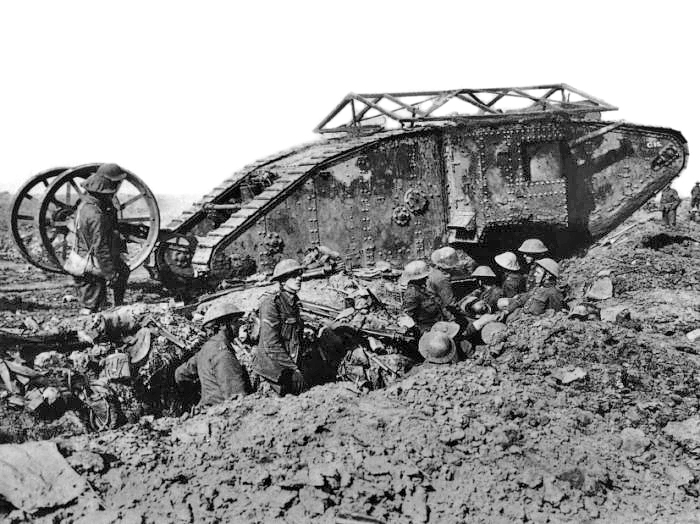
\includegraphics[scale=0.3]{imgs/ws_czolg.jpg}
\caption{Czo�g Mark I u�yty pierwszy raz w bitwie pod Somm� w 1916 r.}
\end{figure}

\begin{figure}[h] \label{czolg_ws}
\centering
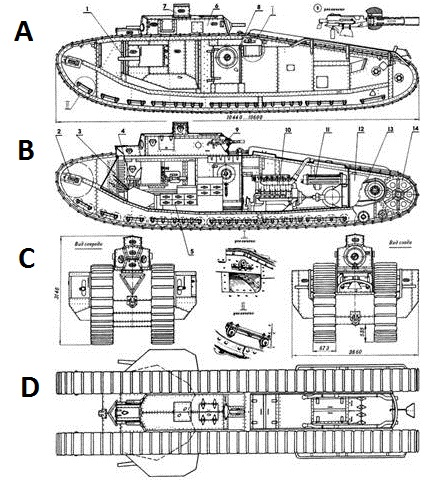
\includegraphics[scale=0.3]{imgs/markviii.jpg}
\caption{Unowocze�niona wersja }
\end{figure}

Zastosowanie czo�g�w pozwoli�o na szybkie zako�czenie konfliktu. Jednak�e pocz�tkowo nie wszyscy dostrzegli w tych pojazdach potencja� militarny. Wynika�o to z faktu, �e by�y one bardzo powolne i s�abo uzbrojone - o niewielkiej warto�ci bojowej. Pocz�tkowo, skoro tylko wojska alianckie posiada�y czo�gi, nie by�o potrzeby montowania w nich wielkiego dzia�a gdy� by�y one przeznaczone do zwalczania piechoty. 

Po zako�czeniu dzia�a� zbrojnych prawie wszystkie pa�stwa przyst�pi�y do projektowania w�asnych pojazd�w bojowych. Zacz�to zatem bra� pod uwag� mo�liwo�� walk typu czo�g-czo�g (a nie jak w przypadku I W� jedynie czo�g-piechota). Efektem tego by�o tworzenie czo�g�w o mo�liwe dobrym pancerzu oraz dziale. Pierwsze konstrukcje tzw. czo�g�w lekkich pojawi�y si� w okolicy 1930 r. Przyk�adem takiego pojazdu mo�e by� radziecki T-26

 

Zosta�y one rozwijane oraz modernizowane. Pocz�tkowo wozy te walczy�y jedynie z piechot� oraz artyleri�. Podczas II wojny �wiatowej dochodzi�o ju� do walk typu czo�g-czo�g co wymusi�o na konstruktorach wyposa�enie ich w pot�ne armaty zdolne do zniszczenia przeciwnika. 

\section{Roboty mobilne}

Robotami mobilnymi nazywamy pojazdy, mog�ce zmienia� swoje po�o�enie w przestrzeni. Dotyczy to nie tylko pojazd�w jezdnych, ale tak�e krocz�cych oraz lataj�cych. Ich g��wn� zalet� jest to ,�e mo�emy nimi sterowa� na odleg�o��. Pozwala to doprowadzi� je do miejsc ,kt�re dla cz�owieka s� niedost�pne lub wykonywa� zadania w �rodowisku zagra�aj�cym naszemu �yciu. Maszyny te s� aktualnie szeroko wykorzystywane przez~:
\begin{itemize}
\item  
s�u�by specjalnie np. wojsko, gdzie mog� pe�ni� rol� bezza�ogowych pojazd�w bojowych lub szpiegowskich,
\item 
agencje kosmiczne, gdzie prowadz� badania badania na innych cia�ach niebieskich (np. eksploracja Marsa przez �azik Curiosity Rover),
\item 
ratownictwo medyczne, gdzie rozwa�a si� wprowadzenie robot�w lataj�cych (typu quadrocopter) do szybkiego dostarczenia pierwszej pomocy w przypadku ataku serca,
\item
geolog�w oraz meteorolog�w do zdalnego dokonywania pomiar�w.
\end{itemize}

\begin{figure}[h]
\centering
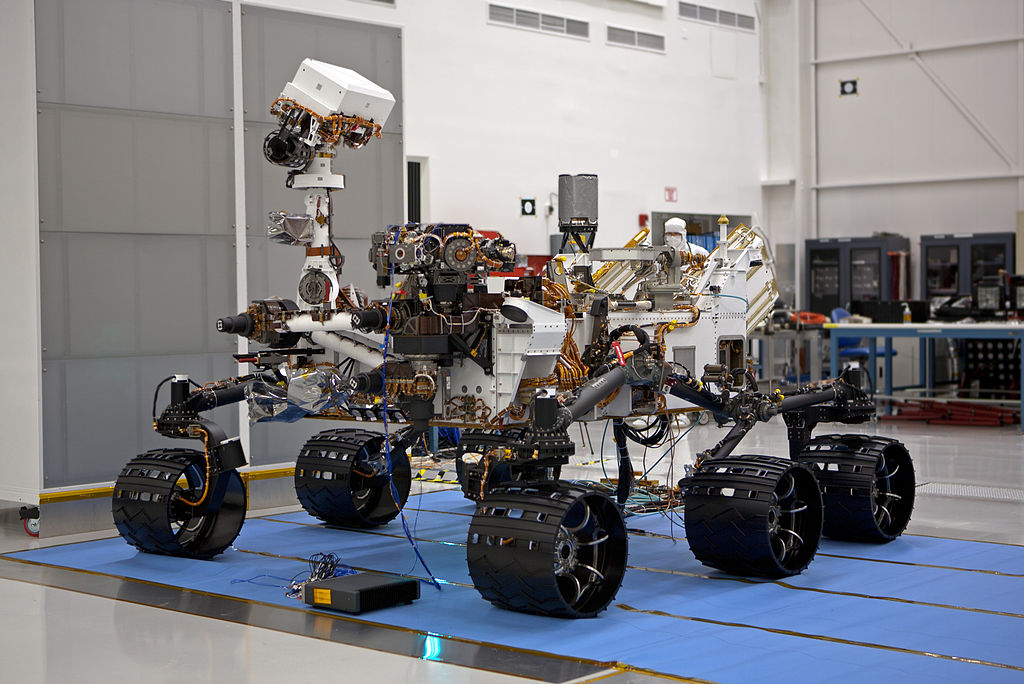
\includegraphics{imgs/curiosity.png}
\caption{Zdj�cie �azika Curiosity Rover jeszcze przed wys�aniem w kosmos.}
\end{figure}

Omawiane maszyny mo�emy dodatkowo wyposa�y� w inteligentne algorytmy pozwalaj�ce na autonomiczn�, czyli pozbawion� wp�ywu cz�owieka, prac�. Dzi�ki wykorzystaniu czujnik�w pomiarowych oraz przy pomocy odpowiedniego oprogramowania mog� one samoistnie rozwi�zywa� niekt�re, z g�ry za�o�one, zadania.

\begin{thebibliography}{9}
% Dodajemy bibliografi� do spisu tre�ci
\addcontentsline{toc}{chapter}{Bibliografia}
\bibitem{SJP}
\emph{S�ownik j�zyka polskiego}, http://sjp.pwn.pl/, (data dost�pu 20.10.2015 r.)

\bibitem{Czech}
\textsc{Leszek Rafi�ski, Aleksandra Bobcow, Andrzej Grono}: \emph{Roboty mobilne z autonomiczn� nawigacj� - stan obecny i perspektywy na najbli�sze lata}. Gda�sk, 2007 r.  

\bibitem{def_robota}
\emph{Teoria robotyki}, http://robotyka.com/, (data dost�pu 21.10.2015~r.)

\bibitem{prawa_robota}
\emph{Prawa robotyki i bunt robot�w}, http://kopernik.org.pl/, (data dost�pu 11.10.2015~r.)

\bibitem{da_vinci}
\textsc{Eugeniusz Olszewski}: \emph{Leonardo da Vinci jako prekursor nauk technicznych}, 1969~r.

\bibitem{robot_squee}
\emph{Squee: The Robot Squirrel}, http://computerhistory.org/, (data dost�pu 22.10.2015~r.)

\bibitem{wojna_pancerna}
\textsc{Tim Ripley}: \emph{Wojna pancerna. Strategia i taktyka}. Warszawa, 2008~r.

\bibitem{programy_rozwoju}
\textsc{Wojciech Zajler, Marek �. Grabania}: \emph{Perspektywiczne programy rozwoju pojazd�w g�sienicowych}. �Szybkobie�ne Pojazdy G�sienicowe�, nr 2, 2003~r.

\bibitem{czolg_przyszlosci}
\textsc{Marek D�browski}: \emph{Czo�g � obecnie i w przysz�o�ci}. �Szybkobie�ne Pojazdy G�sienicowe� nr 2, 2011~r.

\bibitem{kierunek_rozwoju}
\textsc{Wojciech Zajler, Marek �. Grabania}: \emph{Koncepcja modu�owego specjalnego pojazdu wielozadaniowego}. �Szybkobie�ne Pojazdy G�sienicowe� nr 1, 2004~r.

\bibitem{Redlarski}
\textsc{Grzegorz Redlarski, Andrzej Grono, Mariusz D�bkowski}: \emph{Perspektywy rozwoju robotyki}. Gda�sk, 2004~r.

\bibitem{Tadeusiewicz}
\textsc{Ryszard Tadeusiewicz, Przemys�aw Korohoda}: \emph{Komputerowa analiza i przetwarzanie obraz�w}. Krak�w 1997~r.

\bibitem{Malina}
\textsc{Witlod Malina, Maciej Smiatacz}: \emph{Cyfrowe przetwarzanie obraz�w}. Warszawa 2008~r.

\bibitem{Tadeusiewicz_flasinski}
\textsc{Ryszard Tadeusiewicz, Mariusz Flasi�ski}: \emph{Rozpoznawanie obraz�w}. Warszawa 1991~r.


\end{thebibliography}

\listoftables
\listoffigures
\end{document}
